\documentclass[preview]{standalone}
\usepackage{amsmath}
\usepackage{tikz}
\begin{document}
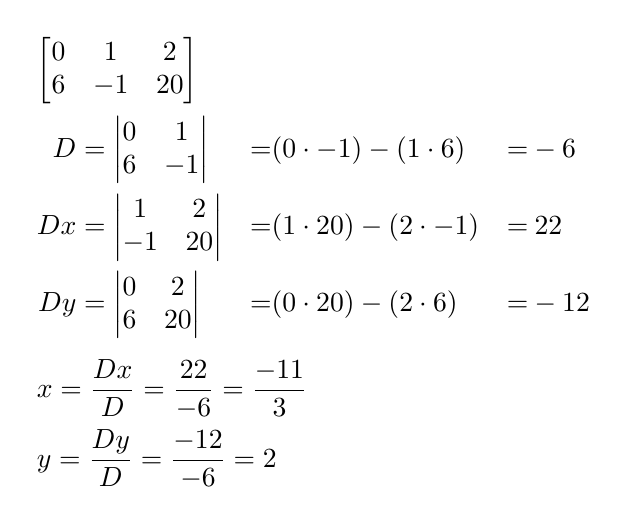
\begin{tikzpicture}
\node[right] at (0, 0) {
  $\begin{bmatrix}0 & 1 & 2 \\6 & -1 & 20 \end{bmatrix}$
};
\node[right] at (0,-2) {
  $\begin{aligned}
    D &= \begin{vmatrix}0 & 1\\ 6 & -1 \end{vmatrix} &= &(0 \cdot -1) - (1 \cdot 6) &= &-6\\
    Dx &= \begin{vmatrix}1 & 2\\ -1 & 20 \end{vmatrix} &= &(1 \cdot 20) - (2 \cdot -1) &=& \:22\\
    Dy &= \begin{vmatrix}0 & 2\\ 6 & 20 \end{vmatrix} &= &(0 \cdot 20) - (2 \cdot 6) &=& -12
  \end{aligned}$};
\node[right] at (0, -4.5){
  $\begin{aligned}
    &x = \frac{Dx}{D} = \frac{22}{-6} = \frac{-11}{3}\\
    &y = \frac{Dy}{D} = \frac{-12}{-6} = 2
  \end{aligned}$};
\end{tikzpicture}
\end{document}